\documentclass[oribibl]{llncs}

\usepackage[T1]{fontenc} \usepackage[utf8]{inputenc} \usepackage[english]{babel}

\usepackage{cite} %Vereinfachung der Referenzen: [1], [2], [3] => [1-3]
\usepackage{makeidx}         % allows index generation

\usepackage{graphicx} \usepackage[cmex10]{amsmath} %mathamatische Formeln 
\usepackage{wrapfig}
\usepackage{placeins}
\usepackage{mathtools}
\usepackage{listings}
\lstset{basicstyle=\small}

\begin{document} \title{Tutorial for usage of the RCLL with the Fawkes Robotics Framework in the Gazebo simulation and YAGI}

\author{Nicolas Limpert} \institute{Fachhochschule Aachen - University of Applied Sciences \and MASCOR Institute}

\maketitle

\begin{abstract}
        This document is supposed to serve as a tutorial for getting started with the software stack provided by the Team Carologistics\footnote{http://www.carologistics.org} in 2015.\\
        Fawkes\footnote{http://www.fawkesrobotics.org} is a robotics framework and fully capable of handling the RoboCup Logistics League (RCLL) \footnote{http://www.robocup-logistics.org}.\\
        The Fawkes implementation meant for the Festo Robotino robots additionally make use of an agent written in the C-Language Integrated Production System (CLIPS).\\
        In this tutorial we instead want to make use of YAGI (Yet Another Golog Interpreter)\footnote{http://yagi.ist.tugraz.at/}.
\end{abstract}

\section{Installation}
Most of this section is gathered from the official documentation at the Fawkes Robotics Website:
\begin{itemize}
        \item \texttt{https://trac.fawkesrobotics.org/wiki/InstallingFawkes}
        \item \texttt{https://trac.fawkesrobotics.org/wiki/FawkesOnFedora}
        \item \texttt{https://trac.fawkesrobotics.org/wiki/Carologistics/Gazsim-Setup-2015}
\end{itemize}
\subsection{Fawkes Dependencies}
It is preferred to make use of Fedora 23 as the time of this writing. Fawkes is mainly developed against Fedora and using Fedora 23 eases up the installation process due to readily available dependencies solved by Fedora's repositories.\\
Although you can of course feel free to have a look at the aforementioned website in order to install it on any other Unix-based operating system.\\
We will consider the installation in Fedora 23 in this tutorial.\\
\\
After a fresh installation of Fedora perform the following\\(refer to ) in order to install the dependencies required to build Fawkes:
\begin{lstlisting}[frame=single]
$ sudo dnf groupinstall development-tools development-libs
$ sudo dnf install fawkes-devenv
$ sudo rpm -e --nodeps tolua++ tolua++-devel
$ sudo dnf install compat-lua compat-lua-devel\
 compat-tolua++ compat-tolua++-devel
\end{lstlisting}

\subsection{ROS (optional)}
For debugging reasons it is recommended to make use of the visualization functionalities of the Robot Operating System called Rviz.\\
To make use of Rviz we have to install the full ROS (the currently used version is "Jade").\\
In order to install ROS (see \texttt{http://wiki.ros.org/jade/Installation/Source}) we want to do the following;
\begin{lstlisting}[frame=single]
$ sudo mkdir /opt/ros/catkin_ws_jade
$ sudo mkdir /opt/ros/jade
$ sudo chown <yourusername>:<yourusername> /opt/ros/*
$ cd /opt/ros/catkin_ws_jade

$ rosinstall_generator desktop_full --rosdistro\
 jade --deps --wet-only\
 --tar > jade-desktop-full-wet.rosinstall
$ wstool init -j8 src jade-desktop-full-wet.rosinstall

$ rosinstall_generator navigation --rosdistro\
 jade --deps --wet-only\
 --tar > jade-navigation.rosinstall
$ rosinstall_generator ar_track_alvar --rosdistro\
 jade --deps --wet-only\
 --tar > jade-ar_track_alvar.rosinstall
$ wstool merge -t src jade-navigation.rosinstall
$ wstool merge -t src jade-ar_track_alvar.rosinstall
$ wstool update -t src
\end{lstlisting}
Where <yourusername> is the username that was given during the installation process of Fedora.\\
Next, build the whole workspace (this can take some minutes):

\begin{lstlisting}[frame=single]
$ cd /opt/ros/catkin_ws_jade
$ ./src/catkin/bin/catkin_make_isolated --install\
 --install-space=/opt/ros/jade -DCMAKE_BUILD_TYPE=Release
\end{lstlisting}

\subsection{Gazebo Models and Plugins}
There are custom models and plugins used by the simulation software Gazebo. E.g. 
\begin{lstlisting}[frame=single]
$ cd ~
$ git clone git@github.com:robocup-logistics/gazebo-rcll.git
$ cd gazebo-rcll/plugins
$ make -j4
\end{lstlisting}

\subsection{LLSF-Refbox}
The RCLL-Refbox \footnote{http://www.robocup-logistics.org/refbox} is the software responsible for handling the game's scores to each of the teams.\\
In order to install it do the following;
\begin{lstlisting}[frame=single]
$ cd ~
$ git clone http://git.fawkesrobotics.org/llsf-refbox.git
$ cd llsf-refbox
$ make -j4
\end{lstlisting}

\subsection{Environmental variables}
In order to promote the LLSF-Refbox installation directory, the Gazebo models and plugins path and so on we have to modify the file \texttt{~/.bashrc}. Insert the following contents at the bottom of this file:
\begin{lstlisting}[frame=single]
source /usr/share/gazebo/setup.bash
source /opt/ros/jade/setup.bash
export FAWKES_DIR=~/fawkes-robotino
export GAZEBO_RCLL=~/gazebo-rcll
export GAZEBO_PLUGIN_PATH=$GAZEBO_PLUGIN_PATH:\
 $GAZEBO_RCLL/plugins/lib/gazebo
export GAZEBO_MODEL_PATH=$GAZEBO_RCLL/models
export GAZEBO_MODEL_PATH=$GAZEBO_MODEL_PATH:\
 $GAZEBO_RCLL/models/carologistics

export LLSF_REFBOX_DIR=~/llsf-refbox
export GAZEBO_WORLD_PATH=\
 1~/gazebo-rcll/worlds/carologistics/llsf.world
\end{lstlisting}

\subsection{YAGI}
YAGI's website \texttt{http://yagi.ist.tugraz.at/} provides access to the release of YAGI including the agent for the LLSF2014.\\
As we are in need of an agent for the LLSF2015 we continued development of the agent to handle the communication used by the Refbox in 2015.\\
The installation can be done in the following way:
\begin{lstlisting}[frame=single]
$ sudo dnf install antlr3-C-devel
$ git clone git@github.com:balamesh/yagi.git
$ cd yagi
$ git checkout nlimpert/llsf2015
$ mkdir build
$ cd build
$ cmake ..
$ make -j4
\end{lstlisting}

\subsection{Fawkes Robotino}
The aforementioned Fawkes Robotics Software-stack is provided by the team Carologistics in a tarball\footnote{https://www.fawkesrobotics.org/blog/2016/02/22/rcll2015-release/}.\\
In order to get / install this Software-stack perform the following:
\begin{lstlisting}[frame=single]
$ wget\
 https://files.fawkesrobotics.org/releases/fawkes-robotino-2015.tar.bz2
$ tar -xjf fawkes-robotino-2015.tar.bz2
$ cd fawkes-robotino
$ make -j4
\end{lstlisting}
\textbf{Important:} After installation make sure you insert the additional skill \texttt{explore\_zone\_wrapped} required to call exploration goals out of YAGI. This skill and the required \texttt{init.lua} is found in the repository \texttt{https://github.com/balamesh/ti\_praktikum\_2016}.\\
You need to copy the files \texttt{explore\_zone\_wrapped.lua} and \texttt{init.lua} to \\\texttt{fawkes-robotino/src/lua/skills/robotino/}.
\newpage

\section{Usage}
\subsection{Starting the simulation}
In order to start the whole simulation including the ROS Environment, the Gazebo simulation software, the LLSF-Refbox and an instance of one Fawkes in order to control the first robot in the simulation do the following;
\begin{lstlisting}[frame=single]
$ cd fawkes-robotino/bin
$ ./gazsim.bash -x start -r -n 1
\end{lstlisting}
There should be 2 windows opening. One of them is a set of terminals including the following:
\begin{enumerate}
        \item \texttt{gazebo including the world-plugin}
        \item \texttt{roscore}
        \item \texttt{refbox-shell}
        \item \texttt{refbox-user-interface}
        \item \texttt{fawkes}
        \item \texttt{fawkes-comm}
\end{enumerate}

\begin{figure}
        \centering
        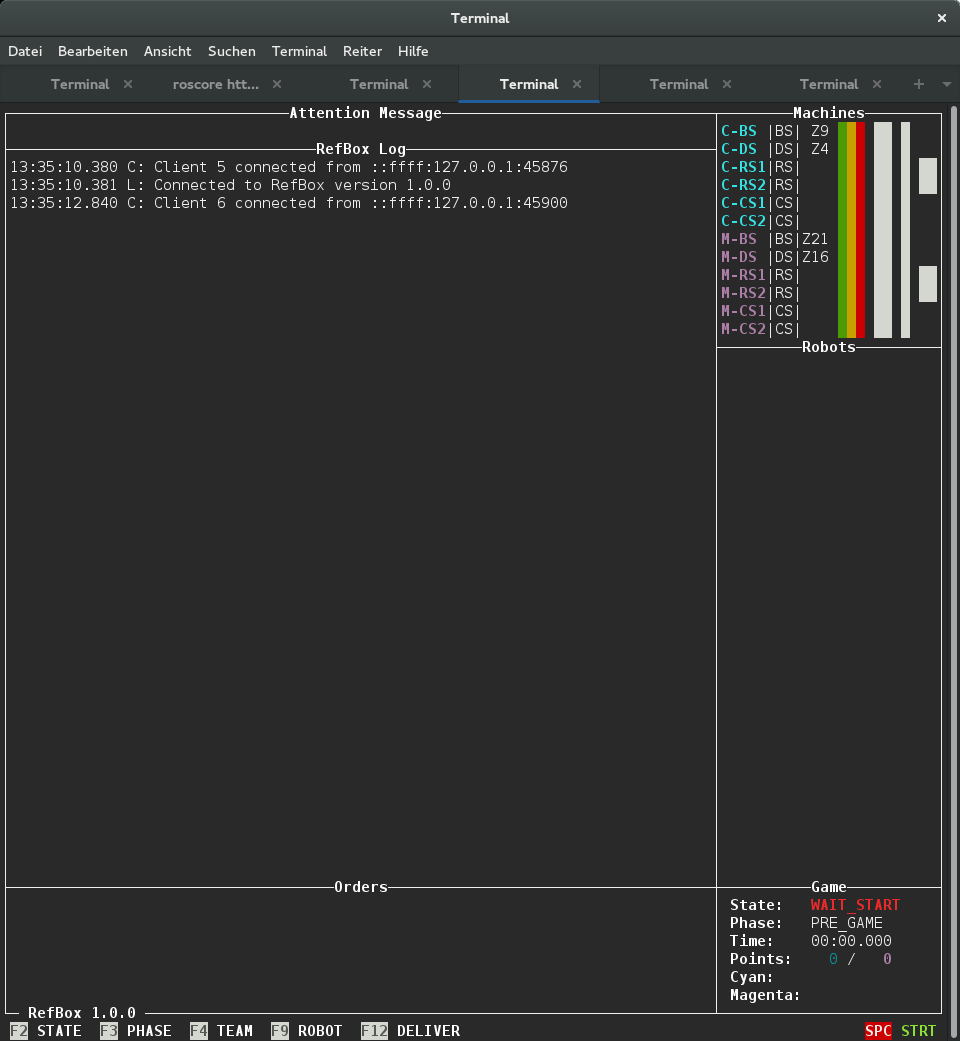
\includegraphics[width=0.5\textwidth]{images/refbox_ui.png}
        \caption{Starting screen of the LLSF-Refbox in the simulation}
        \label{refboxui}
\end{figure}

An example of the refbox starting screen is shown in Figure \ref{refboxui}.
\newpage
\begin{figure}
        \centering
        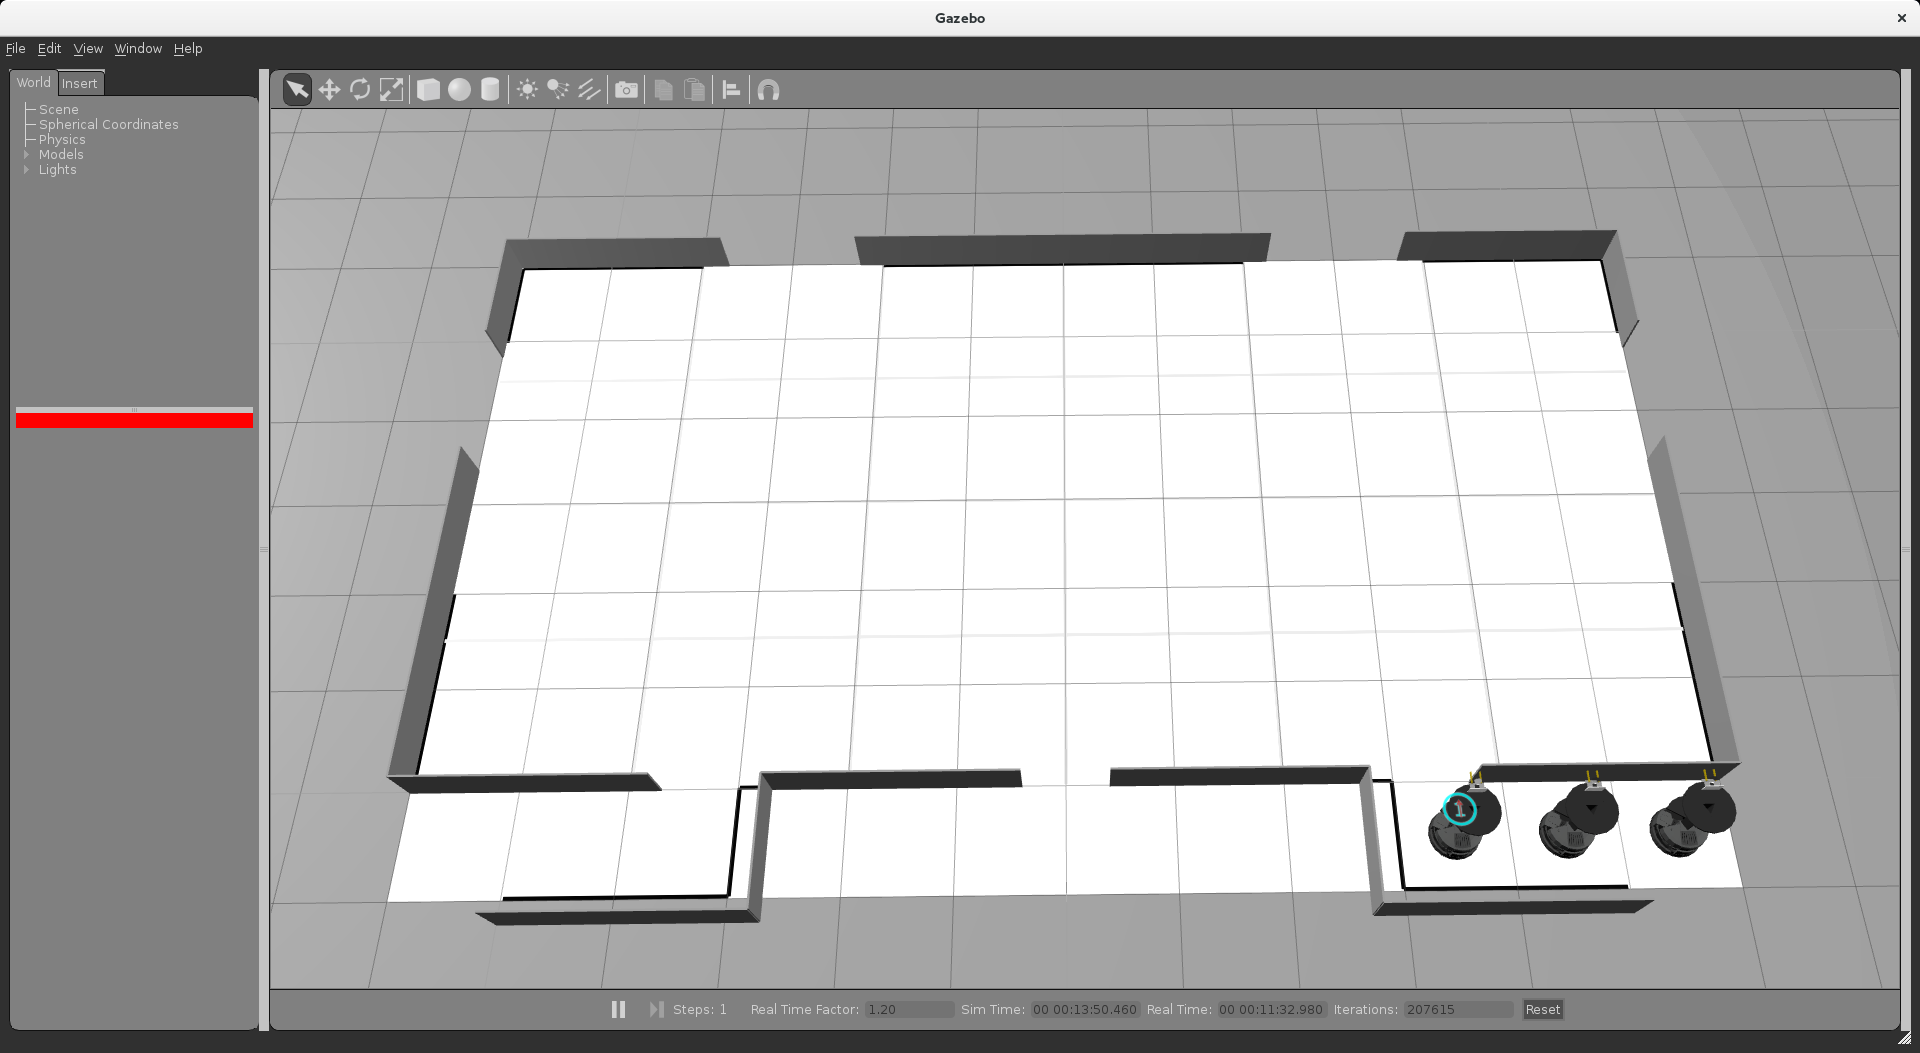
\includegraphics[width=\textwidth]{images/gazebo_start.png}
        \caption{Refbox user-interface}
        \label{gazebostart}
\end{figure}
The other window is the Gazebo simulation environment, shown in figure \ref{gazebostart}.

\subsection{Launching the simulation}
In order to start the game we have to tell the refbox that we first would like to announce the desired team. Do the following:
\begin{enumerate}
        \item Switch to the window shown in figure \ref{refboxui}
        \item Press F4
        \item Press "Return" twice
\end{enumerate}
This sets the team CYAN to "Carologistics".\\
\\
Change the phase from \texttt{PRE\_GAME} to \texttt{SETUP} by pressing \texttt{F3} and afterwards set the game state from \texttt{WAIT\_START} to \texttt{RUNNING} by pressing the \texttt{SPACE}-Key.\\
\textbf{Important:} After changing from the phase \texttt{PRE\_GAME} to \texttt{SETUP} the gazebo-plugin spawns the MPSes. This usually takes a while so be patient until you see all 12 MPSes spawned. A fully launched simulation looks like shown in figure \ref{simulaunchfull}.
\begin{figure}
        \centering
        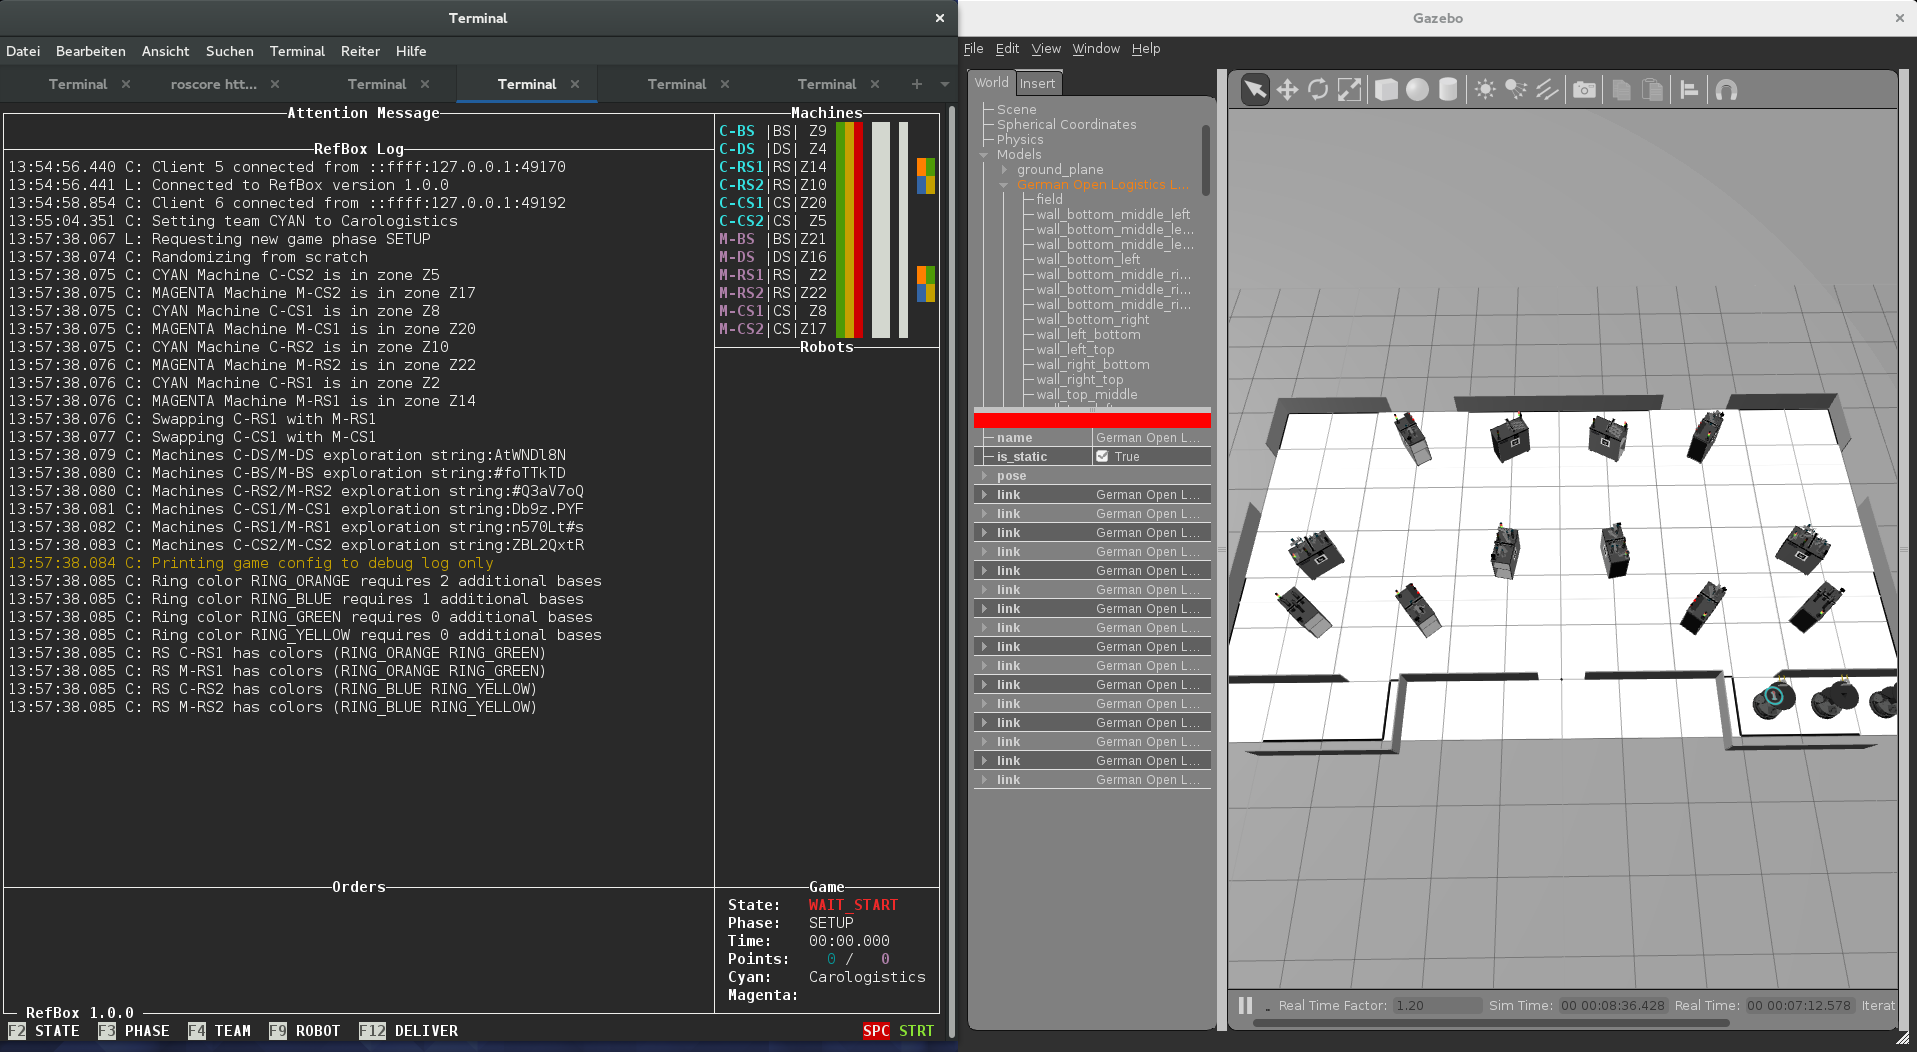
\includegraphics[width=\textwidth]{images/simulaunchfull.png}
        \caption{Exemplary launched simulation including Refbox-UI and Gazebo with spawned MPSes}
        \label{simulaunchfull}
\end{figure}

\end{document}

